%%% PostgreSQL Conference Europe 2013, Dublin, Oct 31, 2013
%%%
%%% A presentation of some tooling I'm building to take care of all the
%%% boring steps of the migration in a single easy and fast step: schema,
%%% handling types and default values, auto-increment and sequences, data,
%%% constraints, indexes.
%%%
%%% That feature set actually works already, only missing is a little glue
%%% and a user language to drive the tool, and that's in good progress
%%% already. The tool would definitely be ready for a full demo at the
%%% conference.
%%%
%%% Obviously the tool licence of choice is "The PostgreSQL Licence".
%%% Actually it's part of the new version of pgloader

\documentclass{beamer}

\usepackage[utf8]{inputenc}

\usepackage{beamerthemesplit}
\usetheme{Boadilla}
%\setbeamertemplate{itemize items}{\checkmark}
\setbeamertemplate{itemize items}[circle]
\beamertemplatetransparentcovered

\usepackage{multicol}

\title{From MySQL to PostgreSQL}
\subtitle{PostgreSQL Conference Europe 2013}
\author{Dimitri Fontaine \texttt{dimitri@2ndQuadrant.fr}
  \linebreak
  \url{@tapoueh}}
\date{October, 31 2013}
\logo{
\includegraphics[height=0.4cm]{2ndQuadrant-cross.png}}

\begin{document}

\frame{\titlepage}

\begin{frame}[fragile]
  \frametitle{Dimitri Fontaine}

  \begin{center}
    \textbf{2ndQuadrant France}
    \linebreak
    PostgreSQL Major Contributor
  \end{center}
  \vfill

\begin{columns}[c]
\column{.75\textwidth} 

  \begin{itemize}
   \item \texttt{pgloader}, \texttt{prefix}, \texttt{skytools}, …
   \item \texttt{apt.postgresql.org}
   \item \texttt{\textbf{CREATE EXTENSION}}
   \item \texttt{\textbf{CREATE EVENT TRIGGER}}
   \item MySQL migration tool, new \texttt{pgloader} version
  \end{itemize}  

\column{.25\textwidth}
\begin{center}
  
\includegraphics[height=7em]{2ndQuadrant-cross.png}
\end{center}
\end{columns}
\end{frame}

\section{pgloader}

\begin{frame}[fragile]
  \frametitle{Migrating from MySQL to PostgreSQL}
  
  \center{A single comand to migrate a whole database}
  \vfill

\begin{verbatim}
load database from mysql://localhost/mydbname
              into postgresql://dim@localhost/pgdbname

with drop tables, truncate, create tables, create indexes,
     reset sequences, downcase identifiers

 set work_mem to '128MB',
      maintenance_work_mem to '512 MB',
     search_path to 'myschema'

cast type datetime to timestamptz drop default using zero-dates-to-null,
     type date drop not null drop default using zero-dates-to-null,
     type tinyint to boolean using tinyint-to-boolean;
\end{verbatim}
\end{frame}

\begin{frame}[fragile]
  \frametitle{Migrating from MySQL to PostgreSQL}
  
  \center{Summary output}
  \vfill

\begin{verbatim}
             table name   imported     errors       time
-----------------------  ---------  ---------  ---------
  station_mapping_cache          0          0      0.035
  test case with errors          5          1      0.138
                    geo          1          0      0.018
 index build completion          0          0        0.0
-----------------------  ---------  ---------  ---------
           create index          7          0      0.082
        reset sequences          1          0      0.023
-----------------------  ---------  ---------  ---------
   Total streaming time          6          1     0.213s
\end{verbatim}
\end{frame}

\begin{frame}[fragile]
  \frametitle{Migrating from MySQL to PostgreSQL}
  
  \center{Source available at \url{http://git.tapoueh.org}}
  \vfill
  \center{\textit{The PostgreSQL Licence}}
\end{frame}

\section{Why}

\begin{frame}[fragile]
  \frametitle{Why Migrating from MySQL to PostgreSQL?}
  
\begin{columns}[c]
\column{.5\textwidth} 

\center{\textbf{MySQL}}
  \vfill

  \begin{itemize}
  \item Storage Engine
  \item Single Application
  \item Data Loss with Replication
  \item Weak Data Types Validation
  \item Either transactions or
  \item Lack of
  \end{itemize}

\column{.5\textwidth} 

  \center{\textbf{PostgreSQL}}
  \vfill

  \begin{itemize}
  \item Data Access Service
  \item Application Suite
  \item Durability and Availability
  \item Consistency
  \item Full Text Search, PostGIS
  \item Proper Documentation
  \end{itemize}
\end{columns}
\end{frame}

\begin{frame}[fragile]
  \frametitle{Free your Data!}

\begin{center}
  
\includegraphics[height=18em]{free-our-open-data.jpg}
\end{center}
\end{frame}

\begin{frame}[fragile]
  \frametitle{Cost Analysis}
  
  \center{What are the costs?}
  \vfill

\begin{columns}
\column{.6\textwidth}

  \begin{itemize}
  \item Migrating the Data
  \item Migrating the Code
  \item Quality Assurance
  \item Opportunity Cost
  \end{itemize}  

\column{.4\textwidth}
\begin{center}
  
\includegraphics[height=7em]{Dollar-sign.jpg}
\end{center}
\end{columns}
\end{frame}

\begin{frame}[fragile]
  \frametitle{Plenty of tools are already available}
  
  \center{Those are not solving the \textit{interesting} problems}
  \vfill

  \begin{itemize}
  \item \texttt{mysql2pgsql} then edit the schema
  \item \texttt{SELECT INTO OUTFILE} on the server, then \texttt{COPY}
  \item MySQL client claims to be sending CSV when redirected
  \item worst case, some \texttt{awk} or \texttt{sed} hackery would do
  \item EnterpriseDB MySQL Migration Wizard
  \item Python and Ruby scripts
  \end{itemize}  
\end{frame}

\begin{frame}[fragile]
  \frametitle{Difficulties when migrating MySQL data}
  
  \center{MySQL dataype input functions are really \textit{sloppy}}
  \vfill

\begin{columns}
\column{.6\textwidth}
  \begin{itemize}
  \item Text, empty string and \texttt{NULL}
  \item Depends on the \texttt{DEFAULT} value
  \end{itemize}
\column{.4\textwidth}
\begin{center}
  
\includegraphics[height=7em]{EmptySet_L.png}
\end{center}
\end{columns}
\end{frame}

\begin{frame}[fragile]
  \frametitle{Difficulties when migrating MySQL data}
  
  \center{Dates and The \textit{Gregorian} Calendar}
  \vfill

\begin{verbatim}
MariaDB [talk]> create table dates(d datetime);
MariaDB [talk]> insert into dates
   values('0000-00-00'), ('0000-10-31'), ('2013-10-00');

MariaDB [talk]> select * from dates;
+---------------------+
| d                   |
+---------------------+
| 0000-00-00 00:00:00 |
| 0000-10-31 00:00:00 |
| 2013-10-00 00:00:00 |
+---------------------+
3 rows in set (0.00 sec)
\end{verbatim}
\end{frame}

\begin{frame}[fragile]
  \frametitle{Difficulties when migrating MySQL data}
  
  \center{MySQL dataype input functions are really \textit{sloppy}}
  \vfill

  \begin{itemize}
  \item \texttt{int}, \texttt{bigint} and \texttt{int(11)}
  \item \texttt{decimal(20,2)} and \texttt{float(20,2)}
  \end{itemize}
  \vfill

\begin{center}
  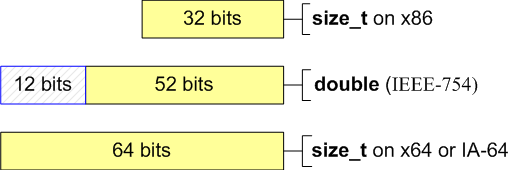
\includegraphics[height=7em]{int-bigint.png}
\end{center}
\end{frame}

\begin{frame}[fragile]
  \frametitle{Difficulties when migrating MySQL data}
  
  \center{No proper \textit{boolean}, but \textit{sets}}
  \vfill

  \begin{itemize}
  \item \texttt{tinyint} and \texttt{boolean}
  \item Inline \texttt{ENUM} and \texttt{SET}
  \item Geometric datatypes input/output...
  \end{itemize}

\begin{columns}
\column{.6\textwidth}
\begin{verbatim}
CREATE TABLE sizes (
    name ENUM('small', 'medium', 'large')
);
\end{verbatim}
\end{columns}
\end{frame}

\section{What}

\begin{frame}[fragile]
  \frametitle{What is the pgloader added value here?}
  
  \center{pgloader is an all-automated declarative migration tool.}
  \vfill

\begin{center}
  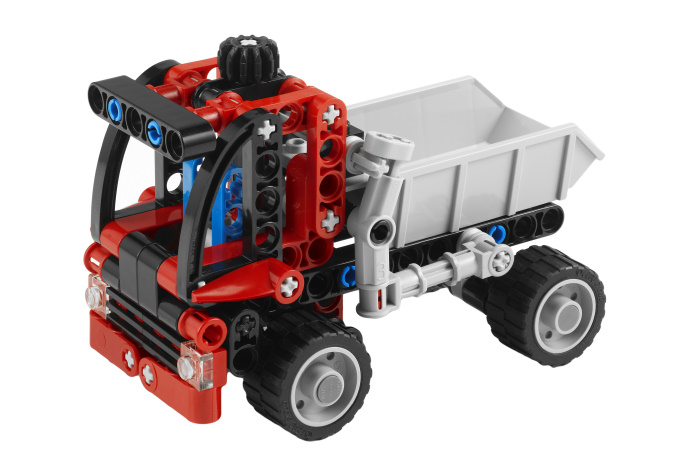
\includegraphics[height=12em]{toy-loader.jpg}
\end{center}
\end{frame}

\begin{frame}[fragile]
  \frametitle{What is pgloader?}
  
  \center{pgloader \texttt{3.x} features}
  \vfill

  \begin{itemize}
  \item We're talking about \texttt{pgloader version "3.0.50.1"} and later.
  \item Load data into PostgreSQL
  \item Using the COPY protocol
  \item Implementing support for bad rows triaging
  \item And flexible data input parsing
  \end{itemize}  
\end{frame}

\begin{frame}[fragile]
  \frametitle{pgloader supported input}
  
  \center{pgloader data source}
  \vfill

  \begin{itemize}
  \item CSV and CSV like files
  \item with per-column \texttt{NULL} and \textit{empty string} definitions
  \item SQLite databases
  \item MySQL databases
  \item dBase \texttt{DBF} binary files
  \item Archives (zip) of CSV or DBF files
  \item Given as an HTTP URL
  \end{itemize}  
\end{frame}

\begin{frame}[fragile]
  \frametitle{pgloader feature set}
  
  \center{pgloader will happily}
  \vfill

  \begin{itemize}
  \item create tables (auto-discovering their schema)
  \item drop tables first if asked
  \item or \texttt{truncate} them
  \item create indexes (auto-discovering them)
  \item in parallel, and in parallel with the next COPY
  \item normalize identifiers (\textit{quote} or \textit{downcase})
  \item reset sequences after the load
  \end{itemize}  
\end{frame}

\begin{frame}[fragile]
  \frametitle{Loading zipped dBase files over HTTP}
  
\begin{verbatim}
LOAD DBF
    FROM http://www.insee.fr/.../.../historiq2013.zip
    INTO postgresql:///pgloader
    WITH truncate, create table
     SET client_encoding TO 'latin1';
\end{verbatim}
\end{frame}

\begin{frame}[fragile]
  \frametitle{Loading CSV data with some \textit{projections}}
  
\begin{verbatim}
LOAD CSV
    FROM INLINE
    INTO postgresql:///pgloader?nulls (f1, f2, f3)
    WITH truncate,
    	 keep unquoted blanks,
         fields optionally enclosed by '"',
         fields escaped by double-quote,
         fields terminated by ','

  BEFORE LOAD DO
   $$ drop table if exists nulls; $$,
   $$ create table if not exists nulls
      (id serial, f1 text, f2 text, f3 text);
   $$;
\end{verbatim}
\end{frame}

\begin{frame}[fragile]
  \frametitle{Some test data}

\begin{verbatim}
"quoted empty string","","should be empty string"
"no value between separators",,"should be null"
"quoted blanks","    ","should be blanks"
"unquoted blanks",    ,"should be null"
"unquoted string",no quote,"should be 'no quote'"
"quoted separator","a,b,c","should be 'a,b,c'"
"keep extra blanks",  test string  , "should be '  test string  '"
\end{verbatim}
\end{frame}

\begin{frame}[fragile]
  \frametitle{Loading several CSV files in a ZIP archive over HTTP, 1/6}
  
\begin{verbatim}
LOAD ARCHIVE
   FROM /Users/dim/Downloads/GeoLiteCity-latest.zip
   INTO postgresql:///ip4r

   BEFORE LOAD DO
     $$ create extension if not exists ip4r; $$,
     $$ create schema if not exists geolite; $$,
     $$ create table if not exists geolite.location
       (
          locid      integer primary key,
          country    text,
          region     text,
          city       text,
          postalcode text,
          location   point,
          metrocode  text,
          areacode   text
       );
     $$,
\end{verbatim}
\end{frame}
\begin{frame}[fragile]
  \frametitle{Loading several CSV files in a ZIP archive over HTTP, 2/6}
  
\begin{verbatim}
     $$ create table if not exists geolite.blocks
       (
          iprange    ip4r,
          locid      integer
       );
     $$,
     $$ drop index if exists geolite.blocks_ip4r_idx; $$,
     $$ truncate table geolite.blocks, geolite.location cascade; $$
\end{verbatim}
\end{frame}

\begin{frame}[fragile]
  \frametitle{Loading several CSV files in a ZIP archive over HTTP, 3/6}
  
\begin{verbatim}
   LOAD CSV
        FROM FILENAME MATCHING ~/GeoLiteCity-Location.csv/
             WITH ENCODING iso-8859-1
             (
                locId,
                country,
                region     null if blanks,
                city       null if blanks,
                postalCode null if blanks,
                latitude,
                longitude,
                metroCode  null if blanks,
                areaCode   null if blanks
             )
\end{verbatim}
\end{frame}

\begin{frame}[fragile]
  \frametitle{Loading several CSV files in a ZIP archive over HTTP, 4/6}
  
\begin{verbatim}
        INTO postgresql:///ip4r?geolite.location
             (
                locid,country,region,city,postalCode,

                location point
         using (format nil "(~a,~a)" longitude latitude),

                metroCode,areaCode
             )
        WITH skip header = 2,
             fields optionally enclosed by '"',
             fields escaped by double-quote,
             fields terminated by ','
\end{verbatim}
\end{frame}


\begin{frame}[fragile]
  \frametitle{Loading several CSV files in a ZIP archive over HTTP, 5/6}
  
\begin{verbatim}
  AND LOAD CSV
        FROM FILENAME MATCHING ~/GeoLiteCity-Blocks.csv/
             WITH ENCODING iso-8859-1
             (
                startIpNum, endIpNum, locId
             )
        INTO postgresql:///ip4r?geolite.blocks
             (
                iprange ip4r
                  using (ip-range startIpNum endIpNum),
                locId
             )
        WITH skip header = 2,
             fields optionally enclosed by '"',
             fields escaped by double-quote,
             fields terminated by ','
\end{verbatim}
\end{frame}

\begin{frame}[fragile]
  \frametitle{Loading several CSV files in a ZIP archive over HTTP, 6/6}
  
\begin{verbatim}
   FINALLY DO
     $$ create index blocks_ip4r_idx
                  on geolite.blocks
               using gist(iprange);
     $$;
\end{verbatim}
\end{frame}

\begin{frame}[fragile]
  \frametitle{Loading several CSV files in a ZIP archive over HTTP}

  \center{1,790,461 rows imported in 18s is about \textbf{100,000 rows/s}}
  
\begin{verbatim}
         table name  imported     errors       time
------------------- ---------  ---------  ---------
            extract         0          0       1.01
        before load         0          0      0.077
------------------- ---------  ---------  ---------
   geolite.location    438386          0     10.352
     geolite.blocks   1790461          0     18.045
------------------- ---------  ---------  ---------
            finally         0          0     31.108
------------------- ---------  ---------  ---------
  Total import time   2228847          0   1m0.592s
\end{verbatim}
\end{frame}

\section{How}

\begin{frame}[fragile]
  \frametitle{How pgloader migrates your data}
  
  \center{pgloader Architecture Choices and features}
  \vfill

\begin{columns}
\column{.6\textwidth}

  \begin{itemize}
  \item Streaming with the COPY protocol
  \item Asynchronous IO with Threads
  \item User Editable Casting Rules
  \item User provided Transforms Functions
  \end{itemize}  

\column{.4\textwidth}
\begin{center}
  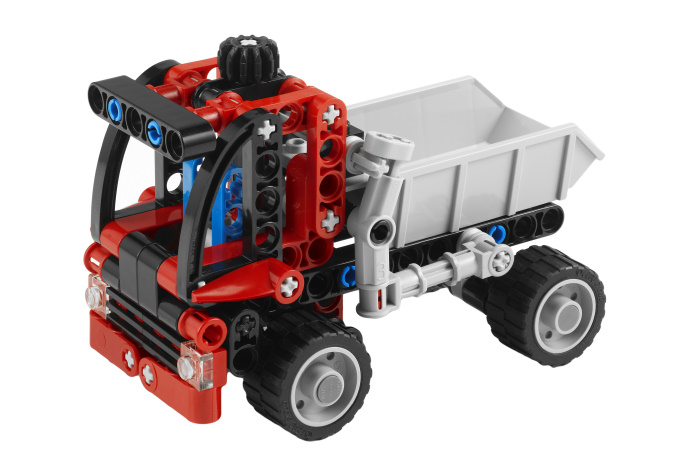
\includegraphics[height=7em]{toy-loader.jpg}
\end{center}
\end{columns}
\end{frame}

\begin{frame}[fragile]
  \frametitle{User Editable Casting Rules}
  
  \center{User Editable Casting Rules}
  \vfill

\begin{columns}
\column{.7\textwidth}
  \begin{itemize}
  \item Used for \textit{schema} conversion
  \item Including \textit{default} values handling
  \item Defines \textit{transform functions}
  \item Those are applied in the streaming \textit{pipeline}
  \end{itemize}
\column{.3\textwidth}
\begin{center}
  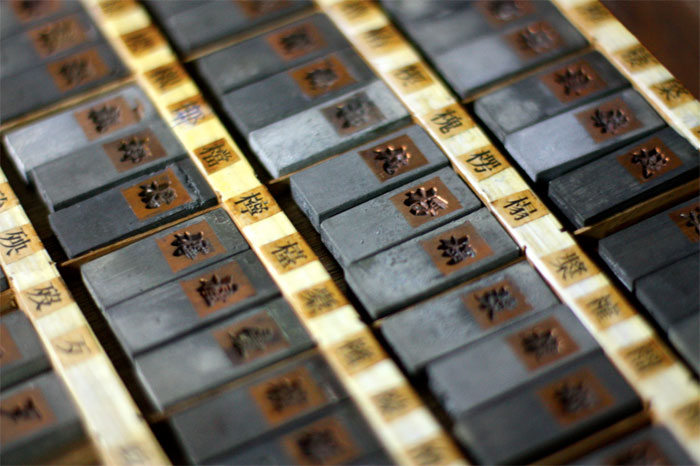
\includegraphics[height=6em]{cast.jpg}
\end{center}
\end{columns}
\end{frame}

\begin{frame}[fragile]
  \frametitle{User Editable Casting Rules}
  
  \center{A detailed example}
  \vfill

\begin{columns}[c]
\column{.5\textwidth}
\begin{verbatim}
type datetime
  to timestamptz
     drop default
     drop not null
     using zero-dates-to-null
\end{verbatim}
\end{columns}
\end{frame}

\begin{frame}[fragile]
  \frametitle{User Editable Casting Rules}
  
  \center{Some use cases}
  \vfill

  \begin{itemize}
  \item Data types with different input/ouput behaviour
  \item \texttt{int(11)} actually is a \texttt{bigint}
  \item \texttt{auto\_increment} means \texttt{serial} or \texttt{bigserial}
  \item \texttt{datetime} almost quite the same as \texttt{timestamptz}
  \item \texttt{NULL} converted as zero dates on \texttt{INSERT}
  \item no proper \texttt{boolean}, only \texttt{tinyint}
  \item inline \texttt{ENUM} support to \texttt{CREATE TYPE}
  \item geometric datatypes \textit{specific} input/output
  \end{itemize}
\end{frame}

\begin{frame}[fragile]
  \frametitle{How pgloader migrates your data}
  
  \center{User provided transformation functions}
  \vfill

  \begin{itemize}
  \item On the fly client-side rewritting of values
  \item Includes rewritting \textit{default} values
  \item A set of transformation functions is included
  \end{itemize}
\end{frame}

\begin{frame}[fragile]
  \frametitle{User provided transformation functions}
  
  \center{Rewriting MySQL data on the fly, when necessary}
  \vfill

  \begin{itemize}
  \item \texttt{zero-dates-to-null} handles \texttt{"0000-00-00"}
  \item \texttt{date-with-no-separator} handles \texttt{"20041002152952"}
  \item \texttt{tinyint-to-bolean}
  \item \texttt{convert-mysql-point} expects \texttt{astext(column)} output
  \item \texttt{astext} used automatically for \texttt{point}
  \end{itemize}
\end{frame}

\begin{frame}[fragile]
  \frametitle{Other necessary transformation}
  
  \center{Text like data and \texttt{NULL} values}
  \vfill

  \begin{itemize}
  \item MySQL returns text \texttt{NULL} as an empty string
  \item pgloader adds \texttt{column is null} output
  \item and process the empty strings depending on \texttt{IS NULL} column
  \end{itemize}
\end{frame}

\begin{frame}[fragile]
  \frametitle{pgloader limitations}
  
  \center{The 80\% rule, Not Implemented Yet are}
  \vfill

\begin{columns}
\column{.6\textwidth}

  \begin{itemize}
  \item Views
  \item Triggers
  \item Foreign Keys
  \item \texttt{ON UPDATE CURRENT\_TIMESTAMP}
  \item Geometric datatypes
  \item Per Column Casting Rules
  \end{itemize}

\column{.4\textwidth}
\begin{center}
  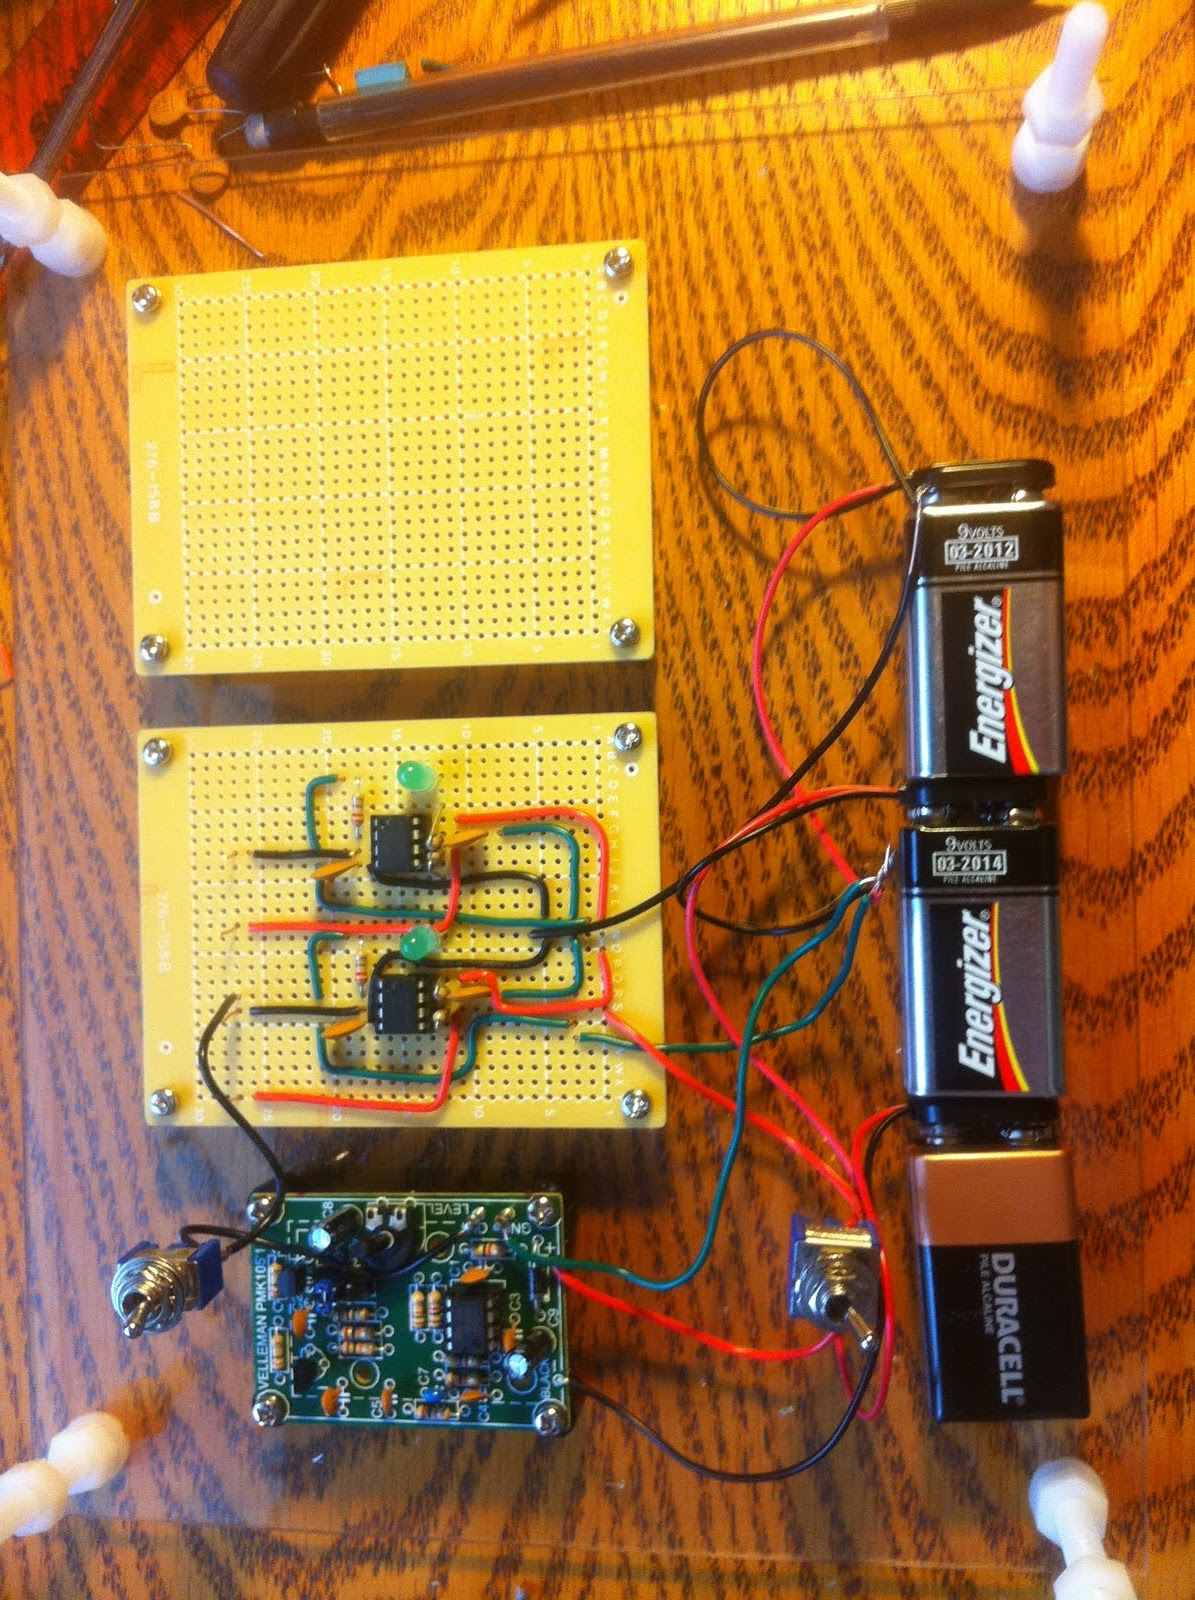
\includegraphics[height=12em]{niy.jpg}
\end{center}
\end{columns}
\end{frame}

\section{Conclusion}

\begin{frame}
  \frametitle{Questions?}

\begin{center}
  Now is the time to ask!
  \vfill
  \begin{center}\url{http://2013.pgconf.eu/feedback}\end{center}
  \vfill

  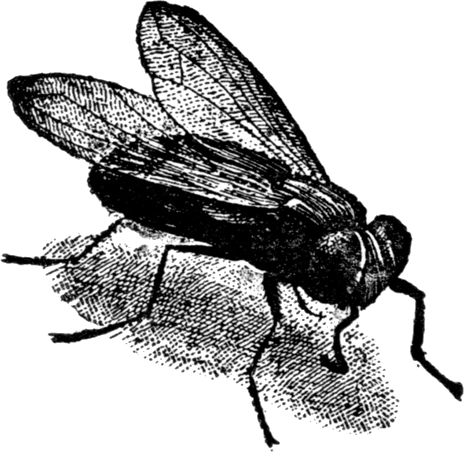
\includegraphics[height=9em]{fly.png}
\end{center}
\end{frame}

\end{document}
